\documentclass{article}

% Language setting
% Replace `english' with e.g. `spanish' to change the document language
\usepackage[english]{babel}

% Set page size and margins
% Replace `letterpaper' with `a4paper' for UK/EU standard size
\usepackage[letterpaper,top=2cm,bottom=2cm,left=3cm,right=3cm,marginparwidth=1.75cm]{geometry}

% Useful packages
\usepackage{amsmath}
\usepackage{graphicx}
\usepackage[colorlinks=true, allcolors=blue]{hyperref}

\title{Exposé Intelligent Agents Geomates Practicals}
\author{Ali Baran Oez, Mohammad Ghassan Aburas, Martin Stuwe, Jendrik Stoltz}

\begin{document}
\maketitle

\section{Main Idea}

The main Idea of our agent is the combination of planning systems and a Large Language Model on different levels of control of the agent. 
With the capability of LLMs of handling loosely defined tasks, the LLM gets tasked to find subgoals / critical points in the level and select one of them as the first goal. As communication is hard with unknown agents in the level,  the Theory of Mind capabilities of LLMs discussed in the lecture are expected to select actions that fit to what the other agent might do in the situation. 

Planning Systems on the other hand offer deterministic results and do not have the hallucination problem of LLMs in complex reasoning tasks ensuring correct plans for reaching goals. Planning systems also have a lower answer latency and are much lighter on resources. 

In our System the LLM therefore only selects subgoals (Lifted Planning) and a PDDL Planner finds a sequence of atomic actions that lead to the subgoal (Grounded Planning). A success or Fail of the plan as well as critical changes in the world affecting the goal are reported to the LLM to react / choose the next subgoal.

\section{Self Localisation}

The self localisation of the agent gets handled by a startup routine that gets executed before giving control to the actual agent code. To find out if the ball or the rectangle are controlled, a "W" command gets send to the game after a wait period derived from the PID of the process. If the ball position changes on the y axis, the agent controls the ball, if the shape of the rectangle changes the agent controls the rectangle. If both changes are observed, the process gets repeated after a random wait interval. When the agent type is determined, control is given to the agent logic.

\section{Agent Structure}

In \ref{fig:architecture} an overview of our agent structure is given. The Agent interacts with the world through a world connector that handles Telnet communication with the game. It takes WASD contol from the Low Level Controller and provides the current world description to the modules of the agent. The Low Level Controller executes a plan of atomar actions the agent can do. Each atomar action consists of a PID controller callback for executing the action, an action description for the PDDL planner containing preconditions and effects as well as state flags indicating a success or fail. The low level controller also checks if something in the world affects a future part of the plan (e.g. other agent in the way, goal diamond gone, atomar action failed) and stops plan execution then. Success and fail of a plan are reported to the LLM with the current world state to find a new subgoal based on the new state.
\begin{figure}[h]
\caption{Architectural Overview}
\label{fig:architecture}
\centering
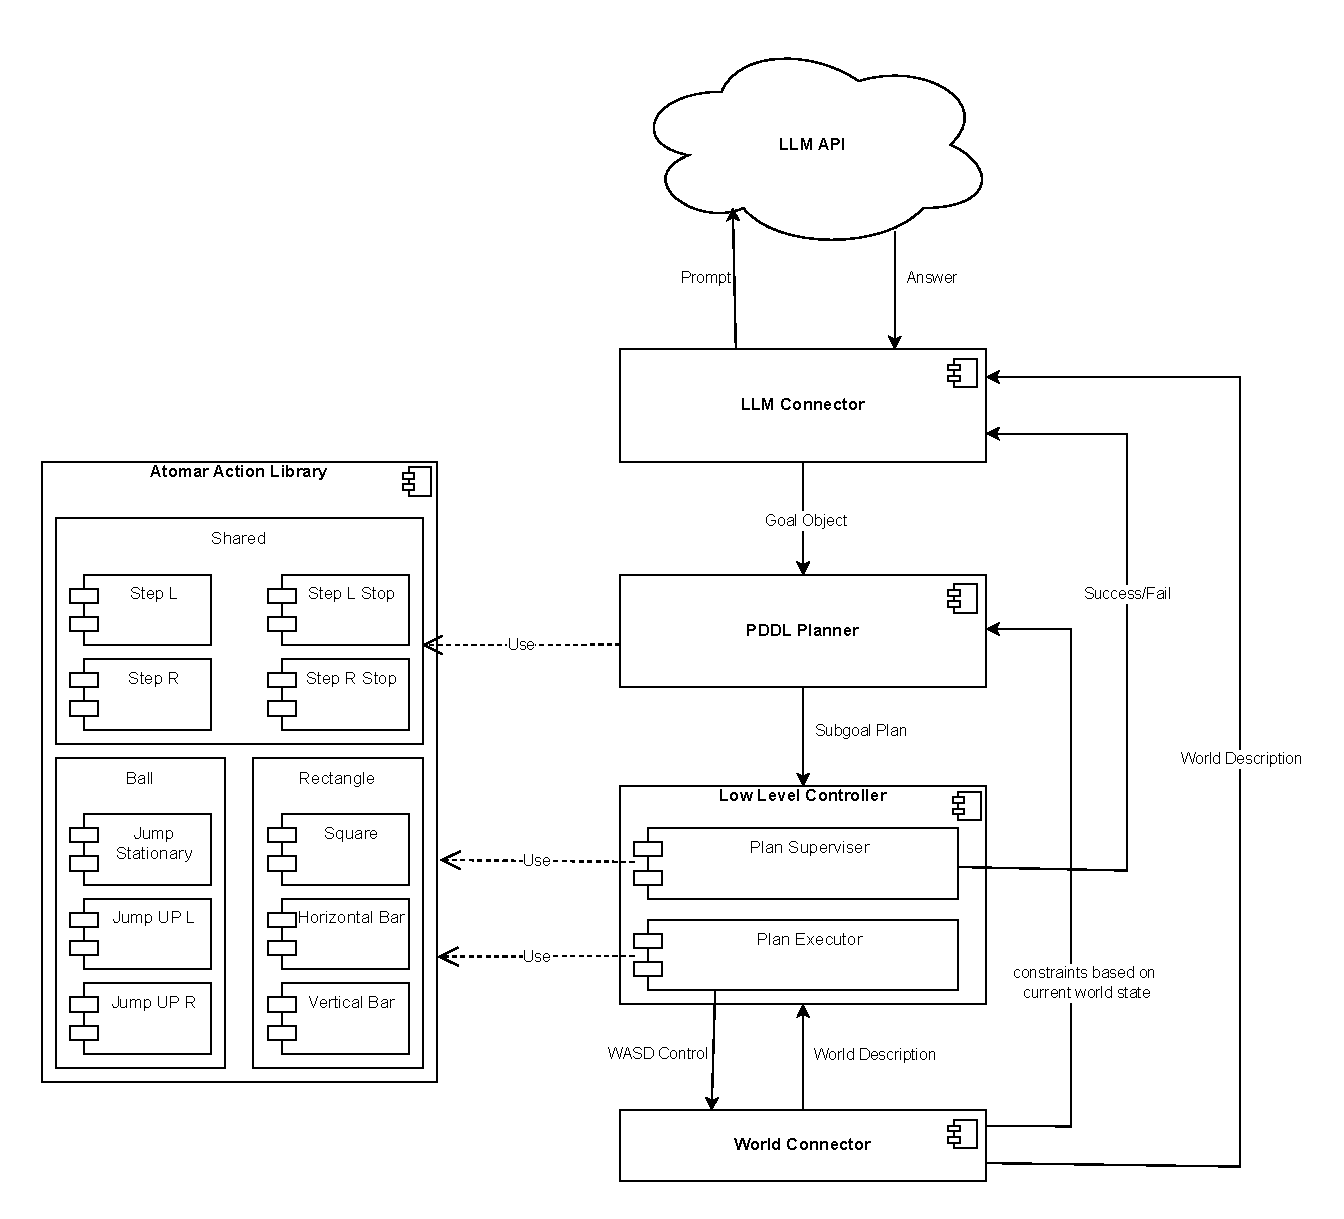
\includegraphics[width=0.7\textwidth]{graphic/IA_llm_agent.pdf}
\end{figure}

\section{Learning through LLM in-context learning}

Requests to the LLM for planning the next tasks are accompanied by a history of actions and their effect. This information can therefore be used to adapt to past behavior of the other agent and success of plans. If the history gets not resetted between levels we hope that the LLM gets better at developing a theory of mind of the other agent and get a better "feeling" of the viability of goals.

\section{Collaboration}

On its own, our agent will only select diamonds as goals and do not offer cooperation. The other player will however be considered in Planning and will be reported to the LLM. If the position of another agent gets considered useful for collecting a goal it can get used. For future development however specific predefined helpful situations could be identified and be proposed to the LLM

\section{Agent Evaluation}

We plan to evaluate our agent in levels containing 
We expect our agent to perform particularly well in levels where It is important to collect diamonds that are not targeted by the other agent like diamonds that are hard to reach and far away for the controlled player but easy to reach and close for the other player. Also cooperation with an agent that offers help (simulated by manual control) could work well. We see problems in Levels containing traps and unrecoverable states as the LLM may have problems understanding the game physics.

\section{Organization}

The Project can be split up in different work packets that can be worked on individually.

\subsection{Software Architecture}
To make the different components of the system work together, a software architecture and a framework defining the structure and communication of the application and the different components has to be defined. The logic and behaviour of the different components will then be added in this framework. The goal of this work package is a working python framework with callbacks for communication between the modules and defined interfaces. It will also include Communication with the simulation via the World connector. The person responsible for this task is Jendrik Stoltz. As integration of the other functionality depends on this task, it has to be worked on early on.

\subsection{Self Localisation}
Ali

\subsection{Low Level Control}
The goal of this work package is the creation of a library of atomic actions for the square and rectangle with the required P(I)D controllers. It will also include a plan executor that will run an action sequence and check for success or fail.
A draft of preconditions and effects of the atomic actions for later use in the planner is also included. The person responsible for this task is Jendrik Stoltz.

\subsection{Connect planner to world and actions}
Martin, Mohammad
\subsection{LLM Setup and Prompt design}
Martin, Mohammad
\subsection{Evaluation}
Ali
\subsection{Deployment}
Everyone Together

\end{document}